\chapter{DESENVOLVIMENTO}

Neste capítulo é apresentada a implementação da aplicação desenvolvida para a realização dos experimentos. São descritas as principais decisões de desenvolvimento, a organização da aplicação, as estruturas \gls{bvh} utilizadas e os métodos empregados para a coleta dos dados. Antes da apresentação da aplicação, são apresentadas algumas decisões tomadas durante o desenvolvimento, principalmente em relação à utilização das estruturas de aceleração e à forma de execução da renderização.

\section{Decisões de Desenvolvimento}

Antes de apresentar a aplicação e os resultados obtidos, é necessário esclarecer algumas decisões tomadas durante o desenvolvimento. Essas decisões foram importantes para definir como as diferentes estruturas \gls{bvh} seriam utilizadas e comparadas, além de estabelecer uma forma de execução que permitisse controlar as principais etapas do processo de renderização.

\subsection{Estrutura da Aplicação}

A aplicação foi construída a partir de uma aplicação já existente, chamada atualmente de \textit{Apotheosis}. De forma resumida, o \textit{Apotheosis} é um motor gráfico desenvolvido para um jogo \textit{open source}, de autoria do autor deste trabalho. Esse motor gráfico foi escolhido por utilizar \textit{Vulkan}, possibilitando maior controle sobre as etapas de renderização e sobre os recursos disponibilizados pelo \textit{hardware}, além de possuir código aberto, ser facilmente compilável por meio de uma \textit{Open Container Initiative Image Format} e já ser conhecido pelo autor deste trabalho \cite{apotheosis}.

O \textit{Apotheosis} já possuía grande parte dos componentes utilizados neste trabalho. O código era baseado principalmente no tutorial de \textit{Vulkan} \cite{vulkan_tutorial} e na documentação do \textit{GLFW} \cite{glfw_docs}. A partir das alterações realizadas para suportar as diferentes estruturas \glspl{bvh} e do aprimoramento das interfaces da aplicação, o código passou a possuir algumas diferenças em relação à versão original.

Uma das principais mudanças foi a redução da compatibilidade com dispositivos que não possuem suporte a alguns recursos utilizados pela aplicação, como \textit{Indexing} e \textit{Buffer Device Address}. Além disso, para a coleta de algumas métricas, também é necessário o suporte a \textit{Host Query Reset}. Dessa forma, a aplicação passou a exigir um conjunto maior de recursos do dispositivo utilizado nos experimentos.

Apesar dessas alterações, a estrutura geral do \textit{Apotheosis} foi mantida. Entre os elementos reaproveitados estão principalmente a organização do projeto, as bibliotecas utilizadas e os arquivos relacionados à compilação. Foram realizadas pequenas adições e alterações nesses componentes para permitir a implementação das estruturas \gls{bvh}, a configuração dos experimentos e a coleta dos dados.

A utilização de uma aplicação já existente também permitiu concentrar o desenvolvimento nas partes relacionadas à comparação das estruturas de aceleração, evitando a necessidade de desenvolver novamente componentes que não fazem parte do objetivo principal deste trabalho.

\subsection{Estruturas de Aceleração}

Apesar de a aplicação utilizar \textit{Vulkan}, as estruturas de aceleração disponibilizadas pela \gls{api} apresentam algumas limitações para os objetivos deste trabalho. Como apresentado anteriormente, as estruturas \gls{blas} e \gls{tlas} utilizadas pelo \textit{Vulkan} possuem sua implementação interna abstraída da aplicação. Dessa forma, não é possível definir diretamente como a estrutura da árvore será organizada ou implementar diferentes estratégias de construção utilizando a estrutura fornecida pela \gls{api} \cite{vulkan_tutorial_acceleration_structures}.

Essa abstração é adequada para aplicações que utilizam o sistema de \textit{ray tracing} fornecido pelo \textit{Vulkan}, porém não atende diretamente ao objetivo de comparar diferentes formas de construção e organização de \glspl{bvh}. Para este trabalho, é necessário possuir controle sobre a estrutura de dados utilizada, permitindo implementar e testar diferentes abordagens, como \gls{bvh}, \gls{lbvh}, \gls{bsah} e \gls{bvh8}.

Outro fator considerado foi a necessidade de utilizar recursos específicos da \gls{api} para realizar a travessia das estruturas fornecidas pelo \textit{Vulkan}. Dessa forma, a utilização dessas estruturas também restringiria a execução da aplicação aos dispositivos que possuem suporte aos recursos necessários para essa abordagem. Neste trabalho, optou-se por manter a utilização do \textit{Vulkan} para as demais etapas da renderização, mas implementar as estruturas \glspl{bvh} utilizadas nos experimentos de forma própria.

Por não serem utilizadas as estruturas de aceleração fornecidas diretamente pelo \textit{Vulkan}, é necessário implementar nos \textit{shaders} o algoritmo responsável pela travessia da \gls{bvh}. Esse algoritmo precisa conhecer a organização dos nós da estrutura, a forma como os dados são armazenados e como acessar os diferentes elementos durante a execução. Essa decisão permite que a mesma aplicação utilize diferentes estruturas e que o processo de travessia seja controlado pelo próprio código desenvolvido para os experimentos.

Essa abordagem também permite separar a estrutura utilizada para armazenar e percorrer a \gls{bvh} da implementação específica das estruturas de aceleração do \textit{Vulkan}. Com isso, as estruturas avaliadas neste trabalho podem ser construídas e armazenadas de acordo com suas próprias características, enquanto a aplicação mantém uma forma comum de execução para realizar a comparação entre elas.

\subsection{Organização da Renderização}

O processo de renderização foi dividido em três etapas principais. A primeira etapa consiste na criação de um \textit{G-buffer} utilizando a técnica de rasterização. Diferentemente de uma utilização convencional da rasterização, nessa etapa são armazenadas informações que serão utilizadas posteriormente durante o processamento dos raios. Entre essas informações estão \textit{position}, \textit{normal}, \textit{albedo}, \textit{material} e \textit{depth}.

O \textit{G-buffer} funciona como uma representação das informações da cena visíveis pela câmera. Dessa forma, a etapa posterior não precisa realizar novamente a busca da geometria correspondente a cada pixel para obter essas informações. A posição, a normal e os demais dados necessários já foram obtidos durante a rasterização e podem ser utilizados pelos \textit{shaders} responsáveis pelo processamento dos efeitos.

Além do \textit{G-buffer} principal, é utilizado um segundo \textit{buffer} com informações semelhantes, porém sem o \textit{depth}. Nesse \textit{buffer} são armazenados materiais considerados transparentes ou que utilizam \textit{blend}, como vidro, água e alguns cristais. Essa separação permite tratar esses materiais de forma diferente durante as etapas posteriores da renderização.

A segunda etapa utiliza as informações armazenadas nos \textit{buffers} para calcular os efeitos de iluminação que dependem da geometria da cena. Entre esses efeitos estão as sombras e os reflexos. É nessa etapa que as estruturas \glspl{bvh} desenvolvidas neste trabalho são utilizadas para realizar a busca das interseções entre os raios e a geometria da cena.

Como a travessia da \gls{bvh} é realizada por meio de uma implementação própria nos \textit{shaders}, o custo dessa etapa pode ser elevado, principalmente quando comparado à utilização das estruturas de aceleração específicas fornecidas pelo \textit{Vulkan}. Por esse motivo, o trabalho concentra a utilização do \textit{ray tracing} em sombras, evitando a inclusão de algoritmos mais complexos de iluminação que poderiam aumentar significativamente o custo da renderização e dificultar a análise do comportamento das estruturas avaliadas.

A terceira etapa é responsável por combinar as imagens geradas nas etapas anteriores e produzir a imagem final apresentada ao sistema. Nessa etapa, os diferentes \textit{buffers} são combinados e podem ser aplicados algoritmos de correção de luminosidade, filtros e outros processos necessários para transformar os resultados intermediários em uma imagem final adequada para apresentação.

\begin{figure}[htb]
	\caption{Organização das etapas da aplicação}
    \centering
    {\parbox{16cm}
        {
            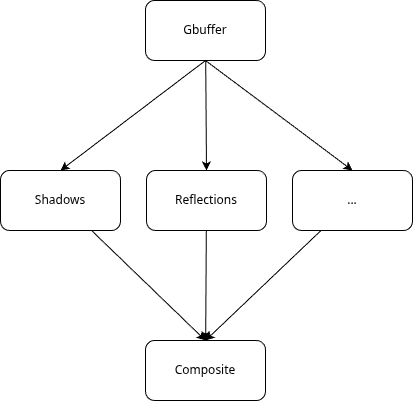
\includegraphics[width=1\textwidth]{images/OrganizacaoDosPipelines.png}
            \label{fig:organizacao_dos_pipelines}
            \hspace{0.0cm}{Fonte: Elaborado pelo autor, utilizando draw.io}
        }
    }
\end{figure}

Neste trabalho, a segunda etapa implementa apenas o cálculo de sombras (\textit{shadows}). Outros efeitos podem ser implementados posteriormente sem a necessidade de alterar as demais etapas da renderização, sendo necessário apenas incluí-los no processo de geração da imagem final, realizado na terceira etapa, também denominada \textit{Composite}. Dessa forma, a organização adotada permite adicionar diferentes efeitos que utilizem as estruturas \glspl{bvh} sem modificar a etapa responsável pela geração do \textit{G-buffer}.

\subsection{Configuração das Estruturas \gls{bvh}}

Para evitar alguns custos associados ao uso de polimorfismo, optou-se pela utilização de \textit{templates} da linguagem C++. \textit{Templates} permitem definir famílias de classes, funções ou tipos que podem ser especializadas a partir dos parâmetros fornecidos. Quando os argumentos são fornecidos, esses parâmetros são substituídos para obter uma especialização específica do \textit{template}, que pode ser instanciada durante a compilação \cite{cppreference_templates}.

Neste trabalho, essa característica é utilizada pelos construtores das estruturas \glspl{bvh}. Os diferentes construtores possuem uma implementação baseada em \textit{templates}, permitindo utilizar diferentes tipos de nós sem a necessidade de criar uma implementação independente para cada combinação. Dessa forma, o tipo de nó e o construtor utilizados podem ser definidos durante a compilação da aplicação.

A seleção da estrutura utilizada é realizada por meio de definições fornecidas ao compilador. Por exemplo, o trecho utilizado para configurar a \gls{blas} verifica se a definição \textit{USE\_BLAS\_BVH8}, \textit{USE\_BLAS\_BSAH} ou \textit{USE\_BLAS\_LBVH} foi fornecida. Caso nenhuma dessas definições esteja presente, é utilizada a implementação padrão da \gls{bvh}. O mesmo processo é aplicado à \gls{tlas}, permitindo selecionar sua estrutura de forma independente da \gls{blas}.

Essa configuração permite realizar diferentes combinações entre as estruturas sem modificar diretamente o código-fonte da aplicação. A escolha pode ser realizada no momento da compilação por meio de parâmetros fornecidos ao \textit{CMake}. Por exemplo, o comando a seguir seleciona a \gls{bvh8} tanto para a \gls{blas} quanto para a \gls{tlas}:

\begin{verbatim}
cmake .. -DCMAKE_CXX_FLAGS="-DUSE_BLAS_BVH8 -DUSE_TLAS_BVH8" \
    -DSHADER_DEFINITIONS="-DUSE_BLAS_BVH8 -DUSE_TLAS_BVH8"
\end{verbatim}

Além de definir essas opções para o código C++, as mesmas definições são fornecidas aos \textit{shaders} por meio do parâmetro \textit{SHADER\_DEFINITIONS}. Isso é necessário porque a construção da estrutura e sua travessia precisam utilizar a mesma organização de dados. Dessa forma, quando uma estrutura é selecionada para a \gls{blas} ou para a \gls{tlas}, a implementação responsável pela travessia nos \textit{shaders} também pode ser configurada para utilizar a estrutura correspondente.

\section{Aplicação Desenvolvida}

Nesta seção são apresentadas as principais partes do desenvolvimento relacionadas à construção e à utilização das estruturas \glspl{bvh}. São descritos o gerenciamento das instâncias, a organização das geometrias e o processo de construção das estruturas de aceleração utilizadas nos experimentos.

\subsection{Criação de instâncias}

As instâncias dos objetos presentes na cena são armazenadas em um vetor de ponteiros. Cada instância pode possuir uma ou mais \textit{submeshes}, que representam partes de uma mesma \textit{mesh} associadas a materiais diferentes. Por exemplo, uma faca pode ser representada por uma única \textit{mesh}, mas possuir uma \textit{submesh} para o cabo de madeira e outra para a lâmina de aço.

Durante a criação do \textit{G-buffer}, essas \textit{submeshes} são organizadas em uma estrutura de dados baseada em \textit{hashmap}, denominada \textit{batch\_map}, que armazena diferentes \textit{batches}. Cada \textit{batch} representa uma \textit{submesh} e contém um vetor com as posições das instâncias que utilizam a mesma geometria, mas podem estar localizadas em posições diferentes da cena. Essa organização permite agrupar chamadas de desenho e utilizar a função \textit{vkCmdDrawIndexed} para renderizar múltiplas instâncias da mesma geometria. Dessa forma, é possível reduzir a quantidade de chamadas de desenho necessárias e a sobrecarga associada ao envio de comandos para a \gls{gpu} \cite{vulkan_vk_cmd_draw_indexed}.

Uma abordagem possível seria criar uma \gls{blas} para cada \textit{submesh}. Isso permitiria associar a geometria e seu material de forma mais direta, facilitando a identificação do material correspondente durante a travessia da estrutura. Entretanto, essa não foi a abordagem adotada neste trabalho. A \gls{blas} é construída por \textit{mesh}, abrangendo suas diferentes \textit{submeshes}. Essa decisão exige que as informações de material sejam mantidas e identificadas durante a travessia da \gls{blas}, pois uma mesma estrutura pode conter primitivas associadas a materiais diferentes.

Durante a criação das instâncias, também é criado um registro denominado \textit{BatchRegistration}. Esse registro mantém a associação entre a instância, sua posição no vetor de instâncias do \textit{batch} e um ponteiro para o próprio \textit{batch}. Dessa forma, é possível atualizar ou remover instâncias sem precisar reconstruir todos os \textit{batches}. Esse mecanismo já existia no \textit{Apotheosis} e foi mantido na aplicação desenvolvida.

Para criar um \textit{batch}, são necessárias as informações presentes na \textit{mesh}, a partir das quais podem ser obtidos os dados utilizados na renderização. Essas informações são gerenciadas pelo \textit{ResourceManager}, responsável por organizar e disponibilizar os recursos utilizados pela aplicação, incluindo aqueles armazenados na \gls{cpu} e na memória da \gls{gpu}. Dessa forma, a aplicação pode consultar os recursos existentes e reutilizá-los quando necessário.

O \textit{ResourceManager} também participa do processo de criação das \textit{meshes}. Como as informações necessárias para a construção da \gls{blas} já estão disponíveis nesse processo, a estrutura de aceleração pode ser construída utilizando os mesmos dados da geometria, evitando a necessidade de realizar uma nova busca pelos recursos correspondentes.

\begin{figure}[htb]
    \caption{Funcionamento dos \textit{batches}}
    \centering
    {\parbox{16cm}
        {
            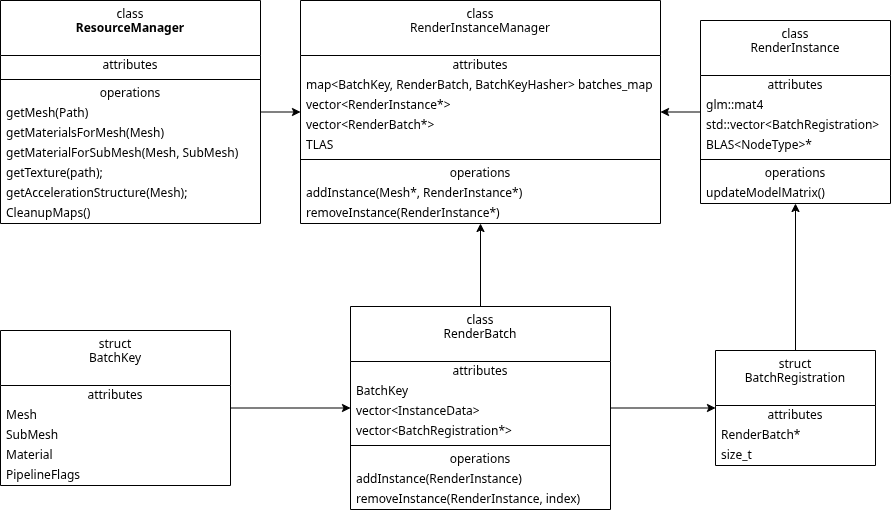
\includegraphics[width=1\textwidth]{images/FuncionamentoDasBatchs.png}
            \label{fig:funcionamento_das_batches}
            \hspace{0.0cm}{Fonte: Elaborado pelo autor, utilizando draw.io}
        }
    }
\end{figure}

\subsection{Criação de luz}

A etapa de criação de luzes apresenta menor complexidade estrutural. Para representar uma fonte de luz na cena, foi criada uma estrutura (\textit{struct}) contendo as principais propriedades necessárias para realizar os cálculos de iluminação nos \textit{shaders}.

\begin{lstlisting}[caption={\textit{Struct} com informações da luz}, label={cod:light_data}]
struct LightData {
    glm::vec3 position;
    float intensity;

    glm::vec3 color;
    float radius;

    Config::LightType type;
    float range;

    float _pad0;
    float _pad1;
};
\end{lstlisting}
\fonte{Elaborado pelo autor (2026).}

A estrutura apresentada no Código \ref{cod:light_data} armazena a posição da luz, sua intensidade e sua cor. Também são armazenados o raio, o tipo da luz e o alcance utilizado durante os cálculos de iluminação. Essas informações permitem que o \textit{shader} determine como a luz deve influenciar os objetos presentes na cena.

A posição é utilizada para determinar a direção e a distância entre a fonte de luz e o ponto que está sendo iluminado. A intensidade define a quantidade de iluminação produzida pela fonte, enquanto a cor permite alterar as componentes de cor da luz. O raio e o alcance são utilizados para controlar a região de influência da luz, evitando que sua contribuição seja aplicada de forma uniforme em toda a cena.

Após a criação e configuração da estrutura, os dados são armazenados em um \textit{buffer} da \gls{gpu}. Esse \textit{buffer} é disponibilizado aos \textit{shaders}, permitindo que as propriedades da luz sejam acessadas durante o processo de iluminação. Assim, a aplicação pode alterar as características da luz no lado da \gls{cpu}, enquanto os \textit{shaders} utilizam essas informações durante a renderização.

Durante a etapa de iluminação, as propriedades da luz são combinadas com as informações armazenadas no \textit{G-buffer}, como posição, normal, material e \textit{albedo}. A partir desses dados, o \textit{shader} calcula a contribuição da luz sobre cada ponto da cena.

No caso das sombras, a posição da luz também é utilizada para determinar a direção do raio que deve ser testado. O raio é então percorrido pela estrutura \gls{bvh} para verificar se existe alguma geometria entre o ponto iluminado e a fonte de luz. Caso uma interseção seja encontrada, o ponto é considerado em sombra e a contribuição direta da luz pode ser descartada.

\subsection{Criação das \glspl{bvh}}

Na aplicação desenvolvida, a \gls{bvh} é construída por \textit{mesh}, e não individualmente para cada \textit{submesh}. Dessa forma, a estrutura de aceleração pode ser associada à instância correspondente. Quando uma nova \textit{mesh} é adicionada e ainda não possui os recursos necessários registrados, a construção da \gls{blas} pode aproveitar o momento em que os dados das primitivas estão disponíveis na \gls{cpu}.

Para permitir a utilização de diferentes implementações de \gls{bvh}, foi necessário definir uma representação comum para os dados utilizados durante a construção. Entre os parâmetros necessários estão os \textit{vertices}, os índices que definem os triângulos e as informações das \textit{submeshes}. Embora a \gls{bvh} seja construída por \textit{mesh}, as informações das \textit{submeshes} ainda precisam ser consideradas para preservar a associação entre as primitivas e seus respectivos materiais. Isso é importante quando um objeto possui mais de um material ou quando algum deles apresenta transparência, utiliza \textit{blend} ou \textit{mask}.

Inicialmente, é criada uma estrutura denominada \textit{PrimitiveRef}, que representa uma primitiva durante o processo de construção da \gls{bvh}. Essa estrutura funciona como uma representação intermediária, permitindo organizar as primitivas antes da criação dos nós da árvore. A partir dessas referências, os algoritmos de construção podem organizar as primitivas e gerar a hierarquia correspondente.

A \textit{PrimitiveRef} também contém uma estrutura \textit{AABB} utilizada para representar os limites espaciais da primitiva. Na estrutura final dos nós, entretanto, os limites são armazenados de outra forma: cada nó mantém as \glspl{aabb} dos seus filhos. Assim, durante a travessia, é possível testar os limites dos filhos antes de acessar os nós correspondentes. Essa organização busca reduzir a quantidade de acessos necessários aos dados dos nós durante a execução do algoritmo.

Outro parâmetro definido durante a construção é a quantidade máxima de triângulos associados a uma instância da \gls{blas}. Nesta implementação, foi estabelecido um limite de quatro triângulos por instância. Essa decisão foi tomada após observar que a árvore apresentava um tamanho elevado, buscando reduzir a quantidade de nós e o espaço necessário para armazenar a estrutura.

Entretanto, esse limite também apresenta desvantagens. Em geometrias pequenas, como cubos e outros objetos com poucos triângulos, diferentes instâncias podem acabar apresentando \glspl{aabb} iguais ou muito semelhantes. Nesses casos, o teste de interseção com as caixas delimitadoras consegue descartar menos primitivas, transferindo uma parcela maior do trabalho para os testes de interseção com os triângulos.

Uma alternativa seria implementar um algoritmo capaz de determinar uma divisão mais adequada para cada geometria, considerando suas características espaciais e a quantidade de triângulos. No entanto, essa estratégia não foi implementada neste trabalho e fica como uma possibilidade para trabalhos futuros.

A estrutura utilizada para representar uma instância da \gls{blas} é apresentada no Código \ref{cod:blas_instance}.

\begin{lstlisting}[caption={\textit{Struct} da instância da \gls{blas}}, label={cod:blas_instance}]
struct BLASInstance {
    uint32_t firstTriangle; //4
    uint32_t triangleCount; //4

    uint32_t materialOffset; //4
    uint32_t pad0; //4
}; //16
\end{lstlisting}
\fonte{Elaborado pelo autor (2026).}

A estrutura armazena o índice do primeiro triângulo associado à instância, a quantidade de triângulos e o deslocamento utilizado para acessar as informações de material. O campo \textit{pad0} é utilizado como preenchimento, contribuindo para manter o tamanho e o alinhamento esperados para a estrutura.

A representação dos nós da \gls{bvh} é apresentada no Código \ref{cod:blas_node}.

\begin{lstlisting}[caption={\textit{Struct} do nó da \gls{blas}}, label={cod:blas_node}]
struct BVHNode {
    AABB childBounds[2]; //128

    uint32_t children[2]; //8

    uint32_t leaf; //4
    uint32_t pad0;//4
}; // 128 + 16 = 144
\end{lstlisting}
\fonte{Elaborado pelo autor (2026).}

Nesse formato, cada nó armazena as caixas delimitadoras dos dois filhos, os índices utilizados para acessá-los e um campo que identifica a condição de folha. O campo \textit{pad0} é utilizado como preenchimento. Essa representação corresponde à estrutura binária utilizada pelas implementações que adotam o tipo \textit{BVHNode}; a \gls{bvh8}, por utilizar nós com maior quantidade de filhos, emprega uma estrutura específica.

Durante a construção da árvore, as referências \textit{PrimitiveRef} são utilizadas para organizar as primitivas e gerar os nós da \gls{bvh}. Após a conclusão desse processo, os dados intermediários são convertidos para o formato utilizado durante a execução, incluindo as instâncias da \gls{blas} e os nós da árvore.

Por fim, os nós e as instâncias são transferidos para dois \textit{buffers} distintos na memória da \gls{gpu}: um destinado às instâncias da \gls{blas} e outro destinado aos nós da estrutura. Embora fosse possível armazenar os dois tipos de dados em um único \textit{buffer}, optou-se por separá-los para simplificar a organização e o acesso aos dados durante a travessia.

O uso de campos de preenchimento, denominados \textit{padding}, em algumas estruturas está relacionado aos requisitos de alinhamento de memória para o acesso aos dados pelos \textit{shaders}. O \textit{Vulkan} define regras de alinhamento para os dados armazenados em \textit{buffers}, que devem ser consideradas na organização das estruturas compartilhadas entre a aplicação e os \textit{shaders} \cite{vulkan_guide_shader_memory_layout}. Além disso, quando é utilizado \textit{Buffer Device Address}, os endereços de memória e os dados acessados precisam respeitar os requisitos de alinhamento aplicáveis \cite{vulkan_guide_bda_alignment}.

\subsection{Criação da \gls{tlas}}

A \gls{tlas} possui um processo de criação semelhante ao da \gls{blas} em alguns aspectos. Primeiramente, são criadas as referências para a \gls{blas} de cada instância que será renderizada. Da mesma forma que na criação da \gls{blas}, também é utilizada a estrutura \textit{PrimitiveRef}. Entretanto, nesse caso, o campo \textit{materialOffset} não é utilizado, pois essa informação é necessária apenas para as instâncias da \gls{blas}.

Utilizando as \textit{PrimitiveRef}, o processo de construção dos nós segue o mesmo princípio utilizado na \gls{blas}. Após a criação dos nós, as \textit{PrimitiveRef} são convertidas em instâncias da \gls{tlas}. Por fim, a \gls{tlas} é transferida para a \gls{gpu} da mesma forma que a \gls{blas}, porém utilizando um \textit{buffer} separado.

\begin{lstlisting}[caption={\textit{Struct} da instância da \gls{tlas}}, label={cod:tlas_instance}]
struct TLASInstance {
    glm::mat4 inverseTransform; // 4*4*32 512

    uint64_t vertexAddress; //8
    uint64_t indexAddress; //8

    uint32_t blasIndex; // 4
    uint32_t nodeOffset; // 4
    uint32_t nodeCount; // 4
    uint32_t instanceOffset; // 4
};
\end{lstlisting}
\fonte{Elaborado pelo autor (2026).}

A estrutura apresentada armazena a transformação inversa da instância, os endereços dos vértices e dos índices da geometria, além das informações necessárias para localizar a \gls{blas} correspondente e os nós associados à instância. O campo \textit{blasIndex} identifica a estrutura utilizada pela instância, enquanto \textit{nodeOffset} e \textit{nodeCount} permitem localizar os nós correspondentes. O campo \textit{instanceOffset} é utilizado para identificar o deslocamento da instância dentro dos dados associados à estrutura.

\section{Construção e travessia das \glspl{bvh}}

Esta seção apresenta o processo utilizado para construir e percorrer os nós das árvores \gls{bvh} implementadas neste trabalho. Inicialmente, é apresentada a implementação da \gls{bvh} binária, utilizada como referência para compreender as demais estratégias. Em seguida, são descritas as alterações realizadas nas abordagens \gls{lbvh}, \gls{bsah} e \gls{bvh8}.

\subsection{\gls{bvh}}

Exceto pela \gls{bvh8}, todas as demais árvores utilizam o mesmo tipo de nó apresentado no Código \ref{cod:blas_node} e seguem essencialmente a mesma forma de travessia. As principais diferenças entre essas estruturas estão relacionadas ao processo de construção. Por esse motivo, inicialmente é apresentada a implementação mais simples, permitindo compreender a organização utilizada e as alterações realizadas nas demais estratégias.

\subsubsection{Construção}

Dentro das funções \textit{BLASInstanceBuilder::build} ou \textit{TLASInstanceBuilder::build}, é chamada a função \textit{BuilderType::build}. No nível responsável pela construção dos nós, a implementação é generalizada, permitindo que a mesma lógica seja utilizada tanto para a \gls{blas} quanto para a \gls{tlas}. O tipo \textit{BuilderType} é definido como um \textit{template} de C++, permitindo utilizar diferentes classes de construção desde que forneçam uma função \textit{build} compatível com os parâmetros esperados. Essa verificação ocorre durante a compilação.

No caso da \gls{bvh}, a função \textit{build} constrói a árvore de cima para baixo (\textit{top-down}), ou seja, partindo da raiz, que contém todas as primitivas, e subdividindo o espaço sucessivamente até alcançar as folhas.

O algoritmo inicia considerando todo o conjunto de primitivas como um único bloco. Para evitar chamadas recursivas, ele utiliza uma pilha para controlar o processo de divisão de forma iterativa. A cada etapa, retira-se um intervalo da pilha e cria-se um nó. Caso esse nó possua um pai, ele é vinculado ao \textit{slot} correspondente do nó superior e sua caixa delimitadora (\gls{aabb}) é calculada.

Quando o nó contém mais de duas primitivas, ele atua como um nó interno: o algoritmo analisa a posição dos centroides das geometrias para escolher o melhor eixo de corte, reordena as primitivas dividindo-as ao meio com o \textit{std::nth\_element} e empilha as duas metades resultantes, esquerda e direita, para serem processadas em seguida. Esse processo de divisão continua até que um grupo passe a ter apenas uma ou duas primitivas. Nessa condição de parada, o nó é finalizado como uma folha (\textit{leaf = 1}) e passa a armazenar diretamente os índices dessas primitivas, encerrando a ramificação daquele ramo.

\subsubsection{Travessia}

A travessia ocorre nos \textit{shaders}. Da mesma forma que as estruturas foram criadas no C++, também é necessário criar suas representações correspondentes nos \textit{shaders}. Foram implementadas algumas funções auxiliares para realizar a travessia, como \textit{intersectTriangle}, utilizada para verificar interseções com os triângulos, e \textit{intersectAABB}, utilizada para verificar interseções com as \glspl{aabb}.

Atualmente, a travessia pode processar mais de um raio de forma iterativa utilizando uma pilha local na memória do \textit{shader}. O fluxo de execução inicia na raiz da árvore, testando a interseção do raio com a caixa delimitadora do nó atual por meio da função \textit{intersectAABB}. Caso o raio não atinja a \gls{aabb}, o ramo inteiro é descartado.

Se houver interseção e o nó for interno, os filhos esquerdo e direito são avaliados e empilhados, priorizando a visita ao filho mais próximo para aumentar a possibilidade de encontrar uma interseção mais próxima antecipadamente. No entanto, essa implementação possui uma limitação: em determinados cenários, o código não consegue realizar a parada antecipada (\textit{early exit}) de forma completa, o que pode obrigar a travessia a explorar nós que poderiam ser descartados.

Por outro lado, caso o nó seja uma folha, o raio é testado diretamente contra as primitivas armazenadas utilizando a função \textit{intersectTriangle}, atualizando o ponto de colisão mais próximo caso haja sucesso. Vale destacar também que, por ser implementado inteiramente por código próprio no \textit{shader}, esse algoritmo não consegue aproveitar as estruturas de aceleração de \textit{hardware} nativas disponibilizadas pelo \textit{driver} da \gls{gpu}, como os \textit{RT cores}.

\subsection{\gls{lbvh}}

A \gls{lbvh} utiliza os códigos de Morton para estabelecer uma ordenação espacial das primitivas antes da construção da hierarquia. Esses códigos representam a posição espacial de cada primitiva por meio de uma sequência de bits obtida a partir das coordenadas de seu centroide. Após a ordenação, as primitivas são organizadas em uma sequência linear, a partir da qual são determinadas as divisões da hierarquia binária \cite{pantaleoni2010hlbvh}.

O processo de construção começa com o cálculo dos limites dos centroides das primitivas. A partir desses limites, o centroide de cada primitiva é normalizado para o intervalo entre zero e um em cada eixo. Essa normalização permite representar as posições independentemente da escala da geometria utilizada.

Após a normalização, cada centroide é convertido em um código de Morton por meio da função \textit{morton3D}. Na implementação desenvolvida, cada coordenada normalizada é quantizada para um valor inteiro entre zero e 1023, utilizando 10 bits por eixo. Em seguida, a função \textit{expandBits} separa os bits de cada coordenada para permitir a intercalação das representações binárias dos eixos X, Y e Z. O resultado é um código de 30 bits que representa a posição tridimensional da primitiva em uma ordem linear. Esse procedimento segue o princípio geral de geração de códigos de Morton descrito na literatura \cite{pantaleoni2010hlbvh}.

O código de Morton é armazenado juntamente com a \textit{PrimitiveRef} correspondente em uma estrutura denominada \textit{MortonPrimitive}. Após a geração desses valores para todas as primitivas, os elementos são ordenados pelo código de Morton utilizando a função \textit{oneapi::tbb::parallel\_sort}. Dessa forma, primitivas com posições espacialmente próximas tendem a ocupar posições próximas na sequência ordenada, embora essa proximidade não seja garantida em todos os casos.

Com as primitivas ordenadas, a construção da árvore é realizada utilizando intervalos dessa sequência. Para determinar a divisão de cada intervalo, a função \textit{determineSplit} utiliza a quantidade de bits iniciais em comum entre os códigos de Morton das primitivas localizadas nas extremidades do intervalo. Essa informação é obtida pela função \textit{commonPrefix}, que compara os códigos por meio da operação \textit{XOR} e determina a quantidade de bits iniciais iguais.

A partir desse prefixo comum, a função \textit{determineSplit} procura uma posição adequada para separar o intervalo em dois grupos. A busca avalia posições candidatas dentro do intervalo e verifica o prefixo comum entre o código da primeira primitiva e o código de cada candidata. Quando o prefixo comum da candidata é maior que o prefixo do intervalo completo, a posição é considerada uma possível divisão. O processo continua até determinar a posição de separação utilizada para criar os dois filhos do nó.

A construção dos nós é realizada de forma paralela por níveis da árvore. Para cada nível, os intervalos que ainda precisam ser divididos são armazenados em estruturas \textit{BuildTask}. Esses intervalos são processados utilizando \textit{oneapi::tbb::parallel\_for}, permitindo determinar as divisões e inicializar os nós de forma paralela. Os novos intervalos gerados são então utilizados como entrada para o próximo nível da construção.

Dessa forma, a implementação utiliza os códigos de Morton para ordenar espacialmente as primitivas e determinar as divisões da hierarquia. Após essa etapa, as \glspl{aabb} são calculadas para os intervalos correspondentes e os nós são organizados em uma estrutura binária. A utilização de operações paralelas durante a geração dos códigos, a ordenação e a construção dos níveis permite explorar o paralelismo disponível durante a construção da \gls{lbvh}.

\subsection{\gls{bsah}}

Enquanto a \gls{bvh} tradicional divide as primitivas simplesmente ao meio usando a mediana, a construção baseada em \gls{sah} (\textit{Surface Area Heuristic}) busca otimizar o custo de interseção do raio, escolhendo o ponto de corte que minimiza a probabilidade de o raio atingir os nós filhos. Para evitar o alto custo computacional de avaliar todas as posições possíveis de corte, esta implementação utiliza uma abordagem compartimentada (\textit{Binned SAH}).

O processo inicia para cada intervalo gerado iterativamente por uma pilha, avaliando os eixos espaciais disponíveis. Em vez de ordenar todas as primitivas individualmente para cada teste, o algoritmo distribui as geometrias em um número fixo de compartimentos (\textit{bins}, por padrão 16) com base nas coordenadas de seus centroides. Para cada compartimento, são acumuladas as caixas delimitadoras (\gls{aabb}) e a contagem de elementos.

Em seguida, o algoritmo calcula prefixos e sufixos cumulativos dos custos de superfície utilizando a heurística de área, avaliando rapidamente o custo combinado de dividir o conjunto em cada ponto de fronteira entre os compartimentos. O ponto de corte que apresenta o menor custo global é selecionado.

Com o eixo e o ponto de divisão definidos, a função \textit{std::partition} reagrupa as primitivas em duas metades com base no compartimento correspondente. Caso ocorra algum desbalanceamento extremo que impeça a partição por compartimentos, o algoritmo recorre a um método de divisão alternativo por mediana (\textit{std::nth\_element}). Por fim, os subintervalos esquerdo e direito são empilhados, calculando-se as \glspl{aabb} finais para cada filho criado.

\subsection{\gls{bvh8}}

A estrutura do nó muda em relação à \gls{bvh} binária tradicional; o nó em si fica maior, mas a ideia principal de hierarquia espacial se mantém.

\begin{lstlisting}[caption={\textit{Struct} do nó da \gls{bvh8}}, label={cod:bvh8_node}]
struct BVH8Node {
AABB childBounds[8]; //256
uint32_t children[8]; //32

uint32_t childCount; //4

uint32_t leaf; //4

uint32_t pad0; //4
uint32_t pad1; //4
}; //256 + 32 + 16
\end{lstlisting}
\fonte{Elaborado pelo autor (2026).}

No que diz respeito à construção (\textit{BVH8Builder}), a principal diferença em relação à \gls{bvh} binária é o fator de ramificação. Enquanto a árvore binária divide o intervalo de primitivas estritamente em duas metades, a \gls{bvh8} particiona o conjunto em até oito partes a cada nível. O algoritmo utiliza uma função recursiva que ordena as primitivas ao longo do eixo de maior dispersão e as distribui uniformemente entre os filhos disponíveis, calculando a \gls{aabb} correspondente para cada um deles. Além disso, as folhas da \gls{bvh8} suportam armazenar até oito primitivas diretamente (\textit{MAX\_LEAF\_PRIMS = 8}), reduzindo a profundidade total da árvore.

No caso específico da travessia, a \gls{bvh8} aproveita essa alta capacidade de ramificação: em vez de testar dois filhos, o algoritmo avalia múltiplas \glspl{aabb}, podendo aproveitar o paralelismo disponível na \gls{gpu}. Como resultado, a árvore fica muito mais rasa, reduzindo a quantidade de níveis que precisam ser percorridos durante o rastreamento dos raios e, consequentemente, a quantidade de acessos aos nós da estrutura.

\section{Configuração dos Experimentos}

Nesta seção são apresentados os procedimentos utilizados para a execução dos testes e o planejamento dos experimentos.

\subsection{Configuração de Hardware e Software}

Os testes foram executados em um ambiente pessoal operando sob o sistema operacional \textit{Arch Linux}, utilizando o \textit{kernel} \textit{Linux} 7.1.11-arch1-1 e o sistema de arquivos \textit{Btrfs} na partição raiz (\textit{/}). O ambiente gráfico utilizado foi o gerenciador de janelas \textit{KDE Plasma} 6.7.4, rodando sobre o protocolo \textit{Wayland}.

Em termos de \textit{hardware}, a máquina é equipada com um processador \textit{Intel Core i5-10600K} (6 núcleos, 12 \textit{threads} operando a uma frequência máxima de 4,10 GHz), acompanhado de 16 GiB de memória \gls{ram}. O processamento gráfico e as execuções de computação paralela via \gls{api} \textit{Vulkan} ficaram a cargo de uma placa de vídeo dedicada \textit{NVIDIA GeForce RTX 5060}, com 8 GiB de memória \gls{vram}, controlada pelo \textit{driver} proprietário da \textit{NVIDIA} na versão 610.57.04 e com suporte à instância \textit{Vulkan} 1.4.357.

\subsection{Preparação para os Experimentos}

O primeiro ponto, e mais simples, é que o \textit{Nsight Systems} não monitora diretamente o uso de memória \gls{ram} do processo. Para obter essa informação, a forma mais prática seria executar um \textit{script} em paralelo durante a execução do teste. Contudo, uma métrica ainda mais útil é o consumo específico de memória das estruturas \gls{bvh}; por isso, em um teste isolado, a aplicação foi configurada para retornar no terminal o tamanho exato ocupado pelas estruturas \gls{blas} e \gls{tlas}.

O \textit{Nsight Systems} consegue capturar a grande maioria dos eventos de forma nativa, mas alguns eventos específicos exigem marcações manuais. Para isso, podem ser utilizados marcadores tanto na \gls{cpu} quanto na \gls{gpu} por meio do \gls{nvtx}. Tratando-se de uma \gls{api} para anotação de código que oferece diversas funcionalidades, foi empregado especificamente o recurso \textit{nvtx3::scoped\_range} \cite{nvidia_nvtx}. Esse componente funciona como um marcador que armazena um título descritivo e finaliza automaticamente a marcação de tempo assim que o bloco de código sai de escopo.

Esse marcador foi utilizado para isolar e medir precisamente o tempo de construção e de transferência das \glspl{bvh} para a \gls{gpu}.

\subsection{Cenas Utilizadas}

A cena é a mesma para todos os experimentos. Ela foi construída de forma rápida, o que significa que não se trata de um cenário realista ou representativo de uma aplicação de produção. A cena consiste em uma junção de várias instâncias dispostas de forma um tanto desordenada, utilizando alguns modelos 3D que não são de autoria própria. A licença de uso estará disponível junto ao código-fonte. Esse modelos vieram de dos usuarios (Eveston - Elite Big Speakerman - Hugo) e (bean(alwayshasbean)), da plataforma \textit{Sketchfab}, utilizada para publicação e compartilhamento de modelos 3D.

Além das múltiplas instâncias, o sistema também conta com animação. A animação compreende o movimento, a rotação e a alteração de escala do modelo completo. A câmera também se movimenta, rotacionando e se afastando do centro da cena em um trajeto circular.

Todas essas alterações garantem que a \gls{tlas} sofra modificações constantes, ainda que sutis, a cada \textit{frame}. Além disso, a movimentação da câmera modifica os dados enviados ao \textit{buffer} e assegura que novas regiões da \gls{tlas} sejam continuamente exploradas.

\subsection{Parâmetros de Execução}

Antes de iniciar os experimentos, realizou-se um levantamento minucioso para identificar quais métricas descritas na literatura poderiam ser efetivamente coletadas e de que forma essa extração seria realizada. Embora algumas métricas específicas tenham permanecido pendentes por limitações de contadores nas ferramentas de análise, o conjunto de dados obtidos ainda supera a variedade encontrada em trabalhos correlatos.

As métricas foram divididas e estruturadas considerando as capacidades do \textit{NVIDIA Nsight Systems} e do \textit{NVIDIA Nsight Graphics}. Métricas de tempo de construção das estruturas de aceleração (\gls{blas} e \gls{tlas}), tempo de quadro na \gls{gpu} (\textit{GPU Frame Time}), utilização dos multiprocessadores de transmissão (\gls{sm}), execuções de \textit{shaders} e transferência de dados via \textit{PCIe} foram extraídas primariamente com o auxílio do \textit{Nsight Graphics}. Em contrapartida, informações de uso de memória \gls{ram} do sistema, consumo energético monitorado via \gls{nvml}, temperatura da \gls{gpu}, trocas de contexto (\textit{context switches}) e atividades nas filas do \textit{Vulkan} foram coletadas por meio do \textit{Nsight Systems}.

Duas métricas merecem destaque metodológico devido ao seu tratamento específico:
\begin{enumerate}
\item \textbf{\textit{Ray Tracing Throughput}:} Como a travessia da \gls{bvh} é realizada diretamente via código próprio em \textit{shaders} (e não pelos núcleos de \textit{ray tracing} dedicados do \textit{hardware}), o rendimento foi calculado relacionando o tempo de travessia ao número total de raios processados por quadro, por exemplo, avaliando resoluções fixas em \textit{Mrays/s}.
\item \textbf{\textit{Warp Divergence}:} Métricas associadas estritamente à divergência de caminhos condicionais dentro de um mesmo \textit{warp} permaneceram pendentes de validação por contadores diretos, evitando o uso de métricas genéricas de ocupação de \gls{sm} como equivalentes.
\end{enumerate}

Para garantir a justiça na comparação de desempenho entre as diferentes estruturas avaliadas (\gls{bvh} binária, \gls{bvh8}, \gls{lbvh} e \gls{bsah}), todas as execuções foram submetidas estritamente às mesmas condições de contorno: a mesma cena animada, idêntico número de instâncias geométricas, mesma resolução de tela, mesma disposição de câmera e a mesma carga de trabalho computacional (\textit{workload}).

\section{Coleta e Tratamento dos Dados}

Nesta seção, descreve-se a metodologia adotada para a extração, o monitoramento e o processamento das métricas de desempenho das diferentes estruturas de aceleração avaliadas.

\subsection{Execução dos Experimentos}

A execução dos testes foi estruturada em duas etapas complementares de perfilamento (\textit{profiling}) para contemplar tanto o comportamento dinâmico e temporal da aplicação quanto os detalhes da renderização gráfica:

\begin{enumerate}
    \item \textbf{Coletas de Longa Duração (\textit{Nsight Systems}):} Os testes voltados a capturar o consumo de recursos globais do sistema, uso de memória \gls{ram} (\textit{Peak RAM Usage}), temperatura, energia e atividades de filas do \textit{Vulkan} foram executados com uma janela de duração de 30 segundos contínuos para cada tipo de \gls{bvh}. Isso permitiu estabilizar as médias e registrar o comportamento da aplicação sob a animação contínua da cena e da câmera.
    \item \textbf{Coletas de Quadros Detalhados (\textit{Nsight Graphics}):} Para a análise minuciosa do \textit{pipeline} gráfico, dos tempos de construção das estruturas de aceleração (\textit{BLAS/TLAS Build Time}) e da execução dos \textit{shaders}, as capturas foram realizadas em momentos específicos. O \textit{profiling} detalhado coletou amostras exatas nos primeiros 2 quadros iniciais e em instantes distribuídos nos segundos 10 e 20 de execução.
\end{enumerate}

Dessa forma, o isolamento dos dados de sistema por meio do \textit{Nsight Systems}, aliado à precisão temporal do \textit{Nsight Graphics}, permitiu mapear com alta fidelidade o impacto de cada variação estrutural de \gls{bvh} sobre a \gls{gpu} e a \gls{cpu}.

\subsection{Coleta das Métricas}

As execuções dos testes para cada tipo de \gls{bvh} foram realizadas em uma mesma sessão experimental, garantindo consistência ambiental. Os artefatos gerados foram organizados em pastas nomeadas de acordo com a respectiva estrutura de aceleração, cujos códigos e arquivos estarão disponíveis no repositório oficial do projeto. Cada diretório contém o executável correspondente, os \textit{shaders} associados e os modelos 3D necessários para a replicação integral dos testes.

Para cada configuração, foram coletados arquivos de registro e relatórios de perfilamento (\textit{profiling}). Especificamente, encontram-se três arquivos com a extensão \textit{.ngfx-capture}, referentes às capturas detalhadas do \textit{Nsight Graphics}, e um arquivo \textit{.nsys-rep}, gerado pelo \textit{Nsight Systems} para a análise global do sistema. Além disso, conforme mencionado anteriormente, o arquivo \textit{bvh\_size\_log.log} armazena os dados textuais referentes ao tamanho em memória de cada estrutura (\gls{blas} e \gls{tlas}).

\subsection{Tratamento dos Dados}

O \textit{Nsight Systems} permite coletar uma grande quantidade de métricas durante a execução da aplicação. Entretanto, a ferramenta é voltada principalmente para a análise da execução ao longo do tempo e para a identificação de problemas de desempenho. Embora forneça os dados necessários para a análise, a apresentação e o tratamento estatístico dessas informações não são suficientes para a análise geral realizada neste trabalho. Dessa forma, foi necessário desenvolver uma etapa adicional para extrair, organizar e analisar os dados obtidos durante os experimentos.

O \textit{Nsight Graphics} apresenta uma abordagem diferente, pois seu objetivo está mais relacionado à análise de um \textit{frame} específico e à visualização das operações executadas durante sua renderização. Dessa forma, os dados obtidos nessa ferramenta são analisados de acordo com as características de cada métrica e com a forma como ela é disponibilizada pela própria ferramenta. Para as métricas obtidas pelo \textit{Nsight Systems}, foi desenvolvido um processo próprio de extração e tratamento dos dados.

A primeira etapa desse processo é realizada pelo \textit{script Python} \textit{extrair\_nsys.py}. O \textit{script} utiliza o executável \textit{nsys} do \textit{Nsight Systems} para processar o arquivo \textit{.nsys-rep} gerado durante a coleta. Como parte desse processo, os dados da execução são disponibilizados em um banco de dados \textit{SQLite}, permitindo consultar as tabelas e informações registradas pelo \textit{Nsight Systems}. A partir dessas informações, o \textit{script} identifica as métricas utilizadas neste trabalho, realiza a extração dos dados correspondentes e gera um arquivo \textit{Excel} denominado \textit{*\_report\_dados.xlsx}. Essa etapa permite separar os dados relevantes das demais informações registradas durante a execução \cite{nsight_systems_post_collection}.

A localização da instalação do executável \textit{nsys} pode variar de acordo com o ambiente utilizado. Por esse motivo, o \textit{script} possui uma variável denominada \textit{NSYS\_DEFAULT}, que pode precisar ser ajustada para apontar para a instalação correspondente do \textit{Nsight Systems}. Essa configuração permite que o mesmo processo de extração seja utilizado em diferentes ambientes de execução.

Após a extração, os dados passam por uma segunda etapa de processamento realizada pelo \textit{script Python} \textit{analisar\_nsys.py}. Esse \textit{script} utiliza o arquivo gerado na etapa anterior e organiza os dados de acordo com cada métrica, calculando informações estatísticas utilizadas posteriormente na análise dos resultados. O resultado é armazenado em outro arquivo \textit{Excel}, denominado \textit{*\_report\_analise.xlsx}.

Para cada métrica, são calculadas informações como unidade de medida, quantidade de amostras, soma, média, mediana, moda, tipo da moda, desvio padrão, valor mínimo e valor máximo. Também são calculadas as mesmas informações após a remoção dos valores considerados \textit{outliers}, permitindo comparar os resultados antes e depois do tratamento dos dados.

A identificação dos \textit{outliers} é complementada pelo cálculo dos limites inferior e superior do intervalo interquartil. Esses limites são utilizados para identificar valores que se encontram fora da faixa considerada para as amostras da métrica. Dessa forma, além dos valores estatísticos originais, o arquivo de análise registra a quantidade e o percentual de \textit{outliers}, bem como os limites utilizados para sua identificação.

O arquivo final contém, portanto, os dados necessários para comparar as métricas obtidas durante os experimentos de forma organizada. Essa separação entre a coleta, a extração e a análise dos dados também permite repetir o processo para diferentes arquivos de execução sem a necessidade de realizar manualmente os cálculos para cada experimento.

Os dois \textit{scripts} são executados para os arquivos de todas as \glspl{bvh} avaliadas neste trabalho. A partir dos arquivos \textit{*\_report\_analise.xlsx} gerados para cada estrutura, é possível reunir os dados e gerar gráficos que facilitam a visualização e a comparação das métricas.

Para isso, foi desenvolvido um terceiro \textit{script Python}, responsável por reunir os arquivos de análise das diferentes \glspl{bvh} e gerar imagens com os gráficos correspondentes. Esses gráficos auxiliam na identificação de diferenças entre as estruturas e facilitam a análise dos resultados obtidos durante os experimentos.

Ambos os \textit{scripts} foram desenvolvidos com o auxílio de inteligência artificial generativa. Desse modo, embora a consistência de todas as métricas apresentadas tenha sido verificada, os \textit{scripts} geram dados adicionais que não foram utilizados neste trabalho, sendo necessária a validação manual desses valores ao menos uma vez para trabalhos futuros.